\section{Deep Learning}
\label{sec:deep_learning}


\subsection{Why Machine Learning}

Machine learning methods try to model either the joint or the marginal distribution of some covariates and some target. In statistics a model is usually explicitly formulated. A typical example could be linear regression. The covariates is decided on, and transformed such that they fit the desired model. The linear regression will yield a parameter vector which can then be interpreted. This interpretation is usually the focus; parameter inference. Example: Does an increase in the minimum salary have a negative effect on BNP per capita. Machine Learning focuses on prediction. That is, the objective is to predict some target conditional on some covariates. The specific model is not necessarily important, instead the focus is on Out-Of-Sample error. These predictive methods lend themselves well where causal inference is not needed. Example: What is the expected consumption on a monthly basis by person with a given set of characteristics. When formulating a traditional econometric method, e.g., OLS, there are standard ways to infer if the model is well specified. In general machine learning does not have the same asymptotic results regarding regularization of a model. Usually sample splitting will be used instead. Take a data set, split the data into two partitions a test set and a training set. First the hyper parameters of the machine learning algorithm is tuned, usually by finding which set of hyper parameters that yield the best performance on the training data. Cross validation is the go-to procedure to optimize the hyper parameters. The final algorithm is only used on the test data set once yielding the out-of-sample performance. Machine learning methods, as mentioned before usually has associated hyper parameters. These are parameters of the model, which is not fitted by training on the data, rather these are specifications of the algorithm before training the model. Much of machine learning is about finding the right hyper parameters and regularizing the model in an intelligent way \parencite{friedman_elements_2001}. Now why is this paper concerned with ML methods? This is due to the fact, that when estimating the value function, or the policy function, one cannot be sure that this follows a linear function. In fact value functions and policy functions might be highly non-linear, which is where machine learning methods shine. Considering that the value function is a conditional expectation: $ \E[Y \mid X=x]$, where $Y$ is the expected cumulative discounted rewards and $X$ is the state implies, that machine learning methods is the appropriate choice for value function approximation. Also, in this case, causal interpretation of the influence of a specific state on the value function is not of interest, rather it's the accuracy of the expected value function\footnote{Obviously, intelligent agents usually do causal inference on their actions. They might not do a certain action exactly because they have some causal notion of how the environment will evolve conditional on their action.}. Deep neural networks has been the standard way to implement reinforcement algorithms, however other machine learning methods can also be used. The reason for deep Learning methods being the standard implementation is the convenient property of online updating of the networks weights. In other words, as more data comes in, the neural network can be incrementally fitted to the new data.

\subsection{Deep Neural Networks}

Deep learning (feed forward networks), which is used in this paper, is in fact just layered non-linear functions. Figure \ref{fig:feedforwardnetwork} illustrates the architecture of a deep neural network\footnote{Figure found at \url{https://upload.wikimedia.org/wikipedia/commons/thumb/c/c2/MultiLayerNeuralNetworkBigger_english.png/381px-MultiLayerNeuralNetworkBigger_english.png}}.

\begin{figure}[ht]
    \centering
    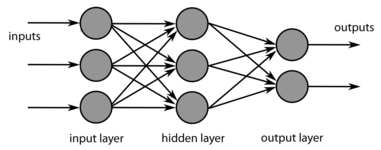
\includegraphics[scale=0.6]{figures/feedforwardnetworkillustration.png}
    \caption{Illustration of Feed Forward Neural Network}
    \label{fig:feedforwardnetwork}
\end{figure}

The network can be described as having an \textit{input layer}, that takes the covariates, $\textbf{x}$. The \textit{hidden layer} makes a transformation of the previous layer. This also implies that a hidden layer, can be followed by an arbitrary number of other hidden layers. Lastly an \textit{output layer} maps the representation of the last hidden layer into the desired output. For classification that could be a one-hot encoding of the classes, and for regression a single real valued scalar.

As illustrated in figure \ref{fig:feedforwardnetwork}, each layer is broken down into smaller cells. The number of cells in each layer corresponds to the width of the layer. The wider the layer the more flexible representation the given layer is capable of doing. The hidden cells work as mentioned by creating a non-linear transformation of the input from last layer:

\begin{equation}
    z_i^{+} = g(\textbf{z}; \theta) = g(\textbf{w}^T \cdot \textbf{z} + b)
\end{equation}

The output of cell \textit{i} is the real valued scalar $z_i^+$. $g$ is the activation function that maps the input into the output. $\textbf{w}$ is the weights of dot product, $\textbf{z}$ is a vector of the outputs from the last layer, and $b$ is bias or the constant in the activation. In that sense the activation looks like a linear regression squashed through an activation function $g$. Multiple different activation functions has been proposed. Originally the logistic function was preferred, but in later years the rectified linear unit activation function has been popular \parencite{goodfellow_deep_2016}:

\begin{equation}
    \textbf{Rectified Linear Unit: }  \max \lcp 0, \textbf{w}^T \cdot \textbf{z} + b \rcp
\end{equation}

The neural network can in other words be considered a function $f$, that takes an input $\textbf{x}$ and maps it to some output $y$, parameterized by $\theta$, which is a collection of all the weights and biases associated with each individual cell.

\subsection{Stochastic Gradient Descent and Optimization}

The neural network is estimated (or trained) by using stochastic gradient descent. This is possible due to the fact, that a neural network can be represented as a set of nested functions, such that the chain rule can be applied. The loss function can in other words be differentiated with respect to the parameter vector $\theta$ as shown below:

\begin{equation}\label{eq:loss_function}
    \frac{\partial}{\partial\theta} \Loss (\textbf{X}, \textbf{Y}, \theta) = \frac{\partial}{\partial\theta} \lp \sum \ell_i \rp = \frac{\partial}{\partial\theta} \lp \sum \lp \hat{Y}_i  - Y_i \rp^2 \rp = \frac{\partial}{\partial\theta} \lp \sum \lp f^{\theta}(X_i)  - Y_i \rp^2 \rp
\end{equation}

In equation \eqref{eq:loss_function} the loss function $\Loss$ is assumed be a mean squared error loss function, in other words a regression problem. The optimization works by minimizing the loss with respect to the parameters $\theta$. In modern neural network architectures it is not unusual to see neural networks have in the excess of a million parameters. The objective function of the optimization cannot be assumed to be convex due to the non-linearity of the activation functions. For this reason deep neural networks is not solved analytically. Instead, gradient descent is used for estimating the parameters of the network. The update rule of the parameters can be described as \parencite{goodfellow_deep_2016}:

\begin{equation}
    \theta \la \theta - \alpha \nabla_{\theta} \Loss(\textbf{X}, \textbf{Y}, \theta)
\end{equation}

So for each step in the algorithm the derivative of the loss function with respect to the parameters can be calculated, and the parameters can be updated by taking a small step in parameter space of size $\alpha$ in the direction that reduces the loss. Stochastic gradient is a response to the fact that it can be computationally expensive to calculate the gradient for the entire data set in each update step. This is important for deep neural networks, since the training period of a large network, even on optimized hardware, can take a very long time, so any speed up for the training is important. In practice this implies that the training data is split into mini batches usually of size 32 to 128. The optimization is then performed on each of the small batches, taking a small step of size $\alpha$ for each step.


